% \documentclass[a4paper,10pt]{article}
\documentclass[review]{siamart}
\usepackage{url}
\usepackage{amssymb}
\usepackage{amsmath}
\usepackage{bm}
\usepackage{stmaryrd}
\usepackage{array}
\usepackage{empheq}
\usepackage{enumitem}
	\setlist{nosep} % or \setlist{noitemsep} to leave space around whole list
\usepackage{color}
%\usepackage{showlabels}
\usepackage{adjustbox}
\usepackage{hyperref}
\hypersetup{
  colorlinks   = true, %Colours links instead of ugly boxes
  urlcolor     = blue, %Colour for external hyperlinks
  linkcolor    = blue, %Colour of internal links
  citecolor   = red %Colour of citations
}
\usepackage[numbers,sort]{natbib}
\usepackage{cleveref}

\newsiamremark{remark}{Remark}


% \newtheorem{lemma}{Lemma}
% \newtheorem{definition}{Definition}
% \newtheorem{theorem}{Theorem}
% \newtheorem{corollary}{Corollary}

\newcommand{\tcb}{\textcolor{blue}}
\newcommand{\tcp}{\textcolor{purple}}
\newcommand{\todo}[1]{\textcolor{red}{[TODO\@: #1]}}

\newcommand{\mdet}{\operatorname{det}}
\newcommand{\madj}{\operatorname{adj}}

% ------------------------------------------------------------------------------------ %
% ------------------------------------------------------------------------------------ %

\newcommand{\TheTitle}{Nonlinear advection-diffusion}
\newcommand{\TheAuthors}{O.A.K}
\headers{Nonlinear advection-diffusion}{\TheAuthors}
\title{{\TheTitle}\thanks{This research was conducted ...
  }}

\ifpdf%
\hypersetup{%
  pdftitle={\TheTitle},
  pdfauthor={\TheAuthors}
}
\fi

% ------------------------------------------------------------------------------------ %
% ------------------------------------------------------------------------------------ %

\begin{document}
\allowdisplaybreaks


% ------------------------------------------------------------------------------------ %
% ------------------------------------------------------------------------------------ %
\section{Summary}

Implemented arbitrarily high-order FD spatial discretizations for the nonlinear, scalar, advection-diffusion problem
\begin{align*}
u_t + \bm{\alpha} \cdot \nabla f(u) = \nabla \cdot ( \bm{\beta} \odot \nabla u ) + s(\bm{x}, t), 
\quad \bm{x} \subset \mathbb{R}^d, 
\quad \bm{\alpha}, \bm{\beta} \in \mathbb{R}^d, 
\quad d \in \{1,2\},
\end{align*}
subject to periodic boundary conditions in space.
\vskip 1ex

\begin{itemize}
\setlength\itemsep{0.5em}
\item Linear, central finite differences for both advection and diffusion terms. Implementation is \underline{not suitable for discontinuities} (e.g., inviscid Burgers). The central discretization of the advection term is also not very well suited for explicit time integration, but we're concerned with implicit, so this doesn't really matter!

\item Serial \& parallel-in-space implementations
\end{itemize}

% ------------------------------------------------------------------------------------ %
% ------------------------------------------------------------------------------------ %
\section{Burgers' convergence study}

\begin{itemize}
\setlength\itemsep{0.5em}
\item Choose $f(u) = u^2$. That  is, we solve
\begin{align*}
\textrm{1D:}\quad &u_t + \alpha u^2_x = \beta u_{xx} + s(x,t),\\
\textrm{2D:}\quad &u_t + \alpha_1 u^2_x + \alpha_2 u^2_y = \beta_1 u_{xx} + \beta_2 u_{yy}  + s(x,y,t),
\end{align*}

\item Set $\delta t = \delta x = \delta y$ (for accuracy reasons). Couple ${\cal O}(p)$ SDIRK time integration with ${\cal O}(p)$ central FD in space. Choose parameters
\begin{align*}
\textrm{1D:}\quad &\alpha = 0.85, \quad \beta =0.3,\\
\textrm{2D:}\quad &\bm{\alpha}= (0.85,1.0), \quad \bm{\beta} =(0.3,0.25).
\end{align*}

\item Manufacture smooth solution then choose $s(\bm{x},t)$ accordingly.

\begin{figure}[htb!]
\centerline{
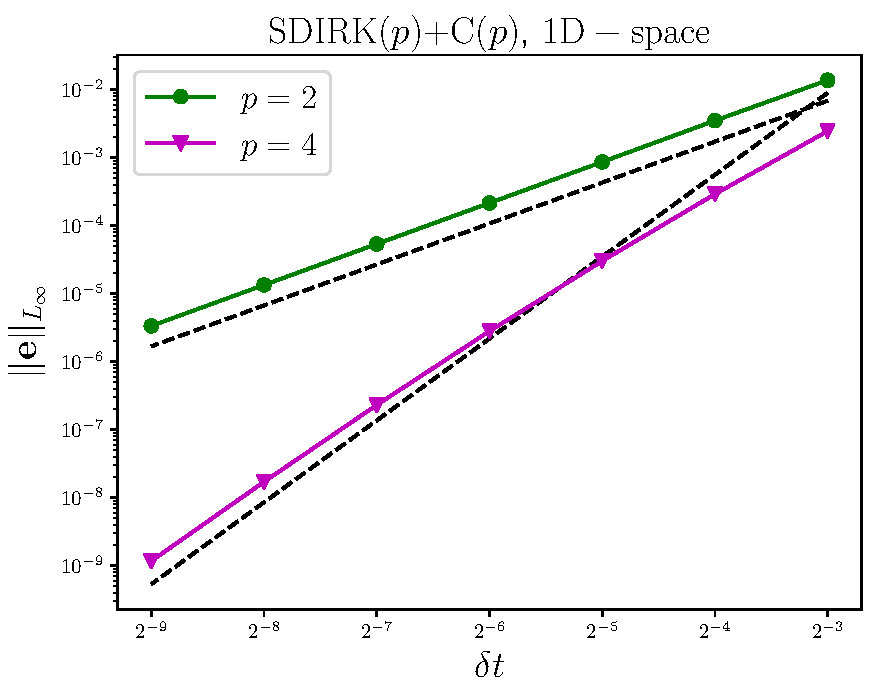
\includegraphics[width = 0.525\textwidth]{../figures/SDIRKd1_ex1}
\quad
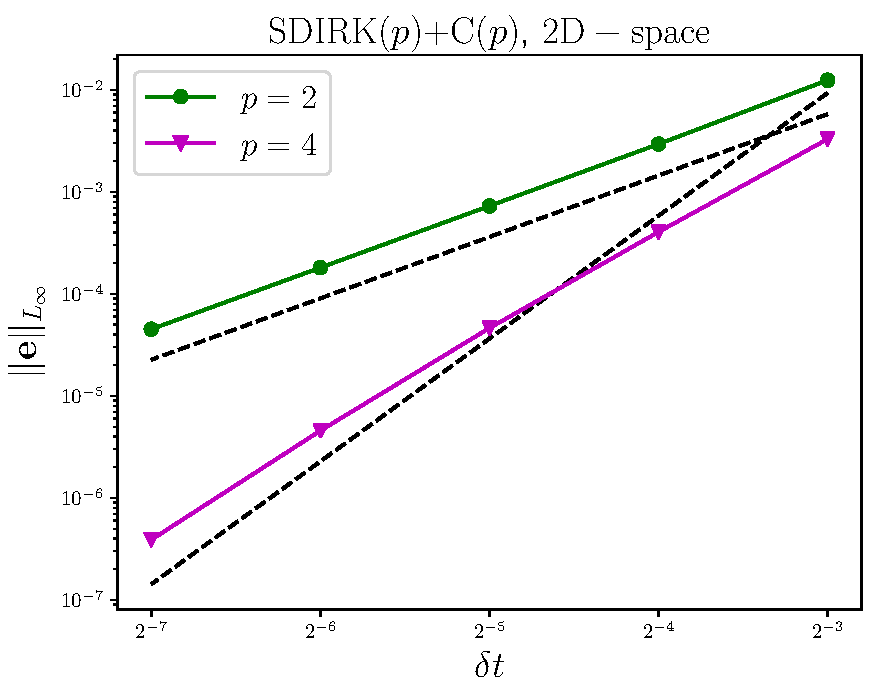
\includegraphics[width = 0.525\textwidth]{../figures/SDIRKd2_ex1}
}
\caption{$L_{\infty}$ errors measured at $t \approx 2$ for smooth manufactured solution to Burgers' equation. Theoretically predicted convergence rates of ${\cal O}(p)$ are shown as dashed black lines. \textbf{Left:} One-spatial dimension. \textbf{Right:} Two-spatial dimensions.
\label{fig:errors}
}
\end{figure}

\item SDIRK time integration requires the solution of nonlinear systems \[\bm{k} + {\cal A}(\bm{u} + \delta t \bm{k}) - {\cal D}(\bm{u} + \delta t \bm{k}) = \bm{s}\] for unknown stage vector $\bm{k}$, where ${\cal A}$ is the nonlinear advection discretization, and ${\cal D}$ the linear diffusion discretization. These systems are solved with full (non-inexact) Newton, preconditioned by GMRES which is preconditioned with AMG (classical AMG for anything but small diffusivities, otherwise with AIR).
\end{itemize}





% ------------------------------------------------------------------------------------ %
% ------------------------------------------------------------------------------------ %
\section{Example problem}

\begin{itemize}
\setlength\itemsep{0.5em}
\item Put source $s = 0$, and choose $\bm{\alpha}=(1.0,1.0)$, $\bm{\beta}=(0.075,0.075)$. 

\item Solutions for linear advection, and Burgers' advection are shown in Figure \ref{fig:example}.

\item Observe qualitatively different behaviour: Linear PDE propagates and dissipates initial condition isotropically. Nonlinear PDE also dissipates, but steepens wave front in direction of velocity vector and rarefies it (spreads it out) in direction opposite to velocity vector.

\item Newton and GMRES seem to converge quite quickly for most of the problems I've looked at. Except some issues with AIR for moderate values of $\delta t/ \delta x$. See fast (quadratic) Newton convergence for the nonlinear PDE in Figure \ref{fig:solves}.
\end{itemize}

\begin{figure}[htb!]
\centerline{
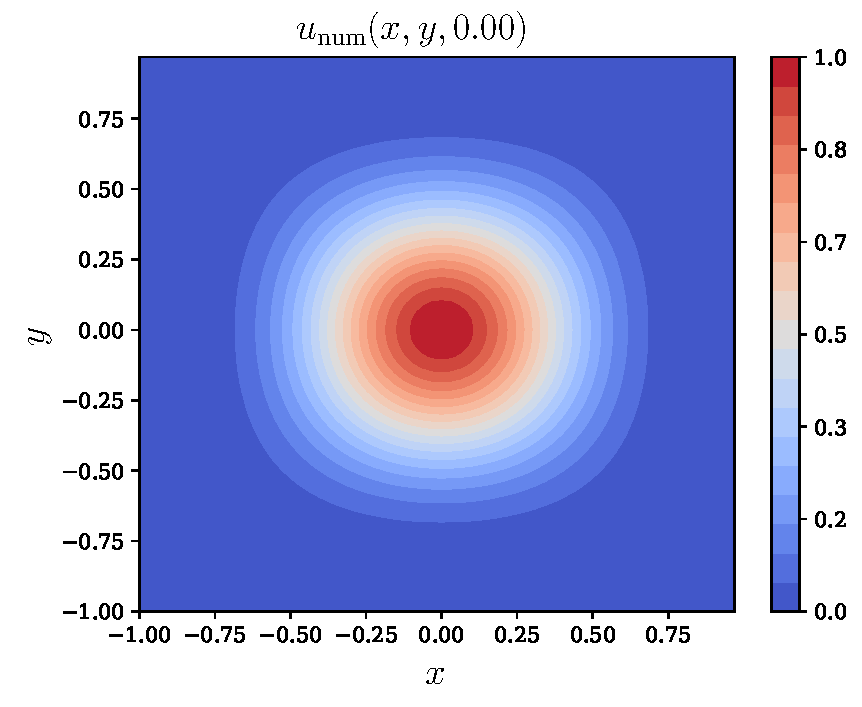
\includegraphics[width = 0.6\textwidth]{../figures/ic}
}
\centerline{
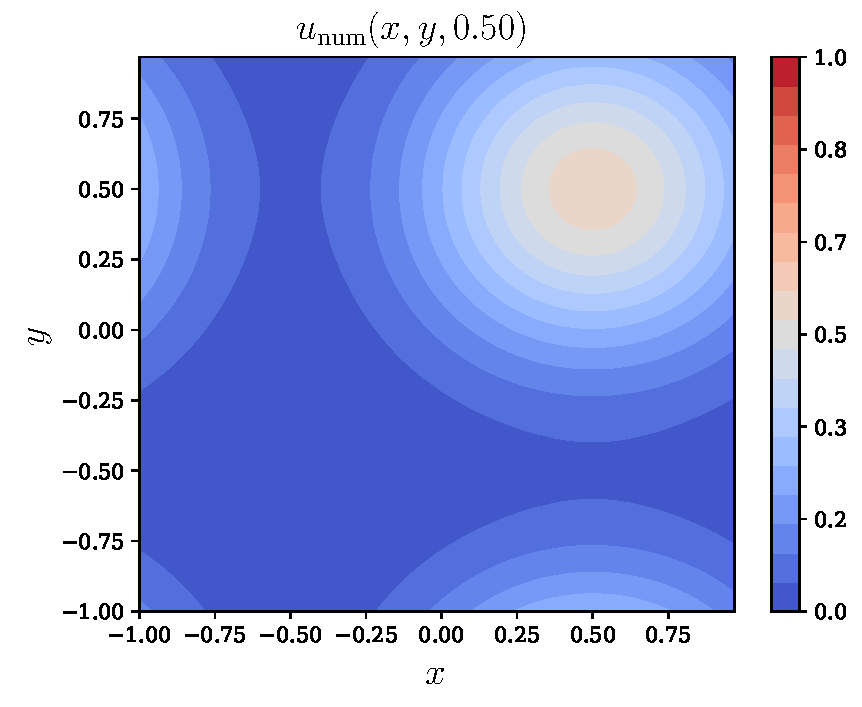
\includegraphics[width = 0.6\textwidth]{../figures/linear}
\quad
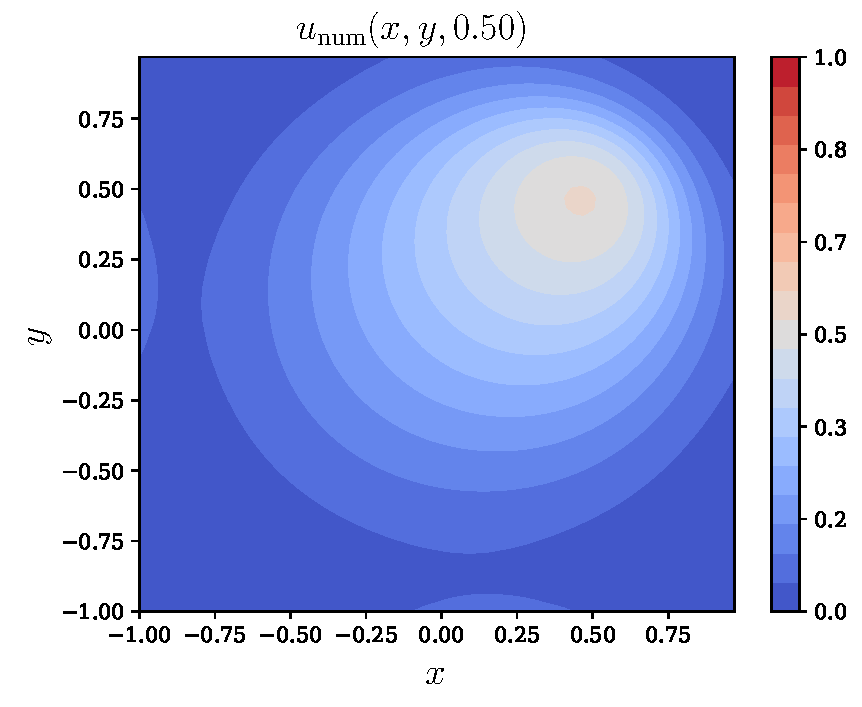
\includegraphics[width = 0.6\textwidth]{../figures/nonlinear}
}
\caption{\textbf{Top:} Initial condition, $u(x,y,0)= \sin^4 \big(\tfrac{\pi}{2}(x-1) \big) \sin^4 \big(\tfrac{\pi}{2}(y-1) \big)$. \textbf{Bottom left:} Solution of linear PDE, $f(u)=u$, at $t=0.5$. \textbf{Bottom right:} Solution of nonlinear PDE, $f(u)=u^2$, at $t=0.5$.
\label{fig:example}
}
\end{figure}


\begin{figure}
\centerline{
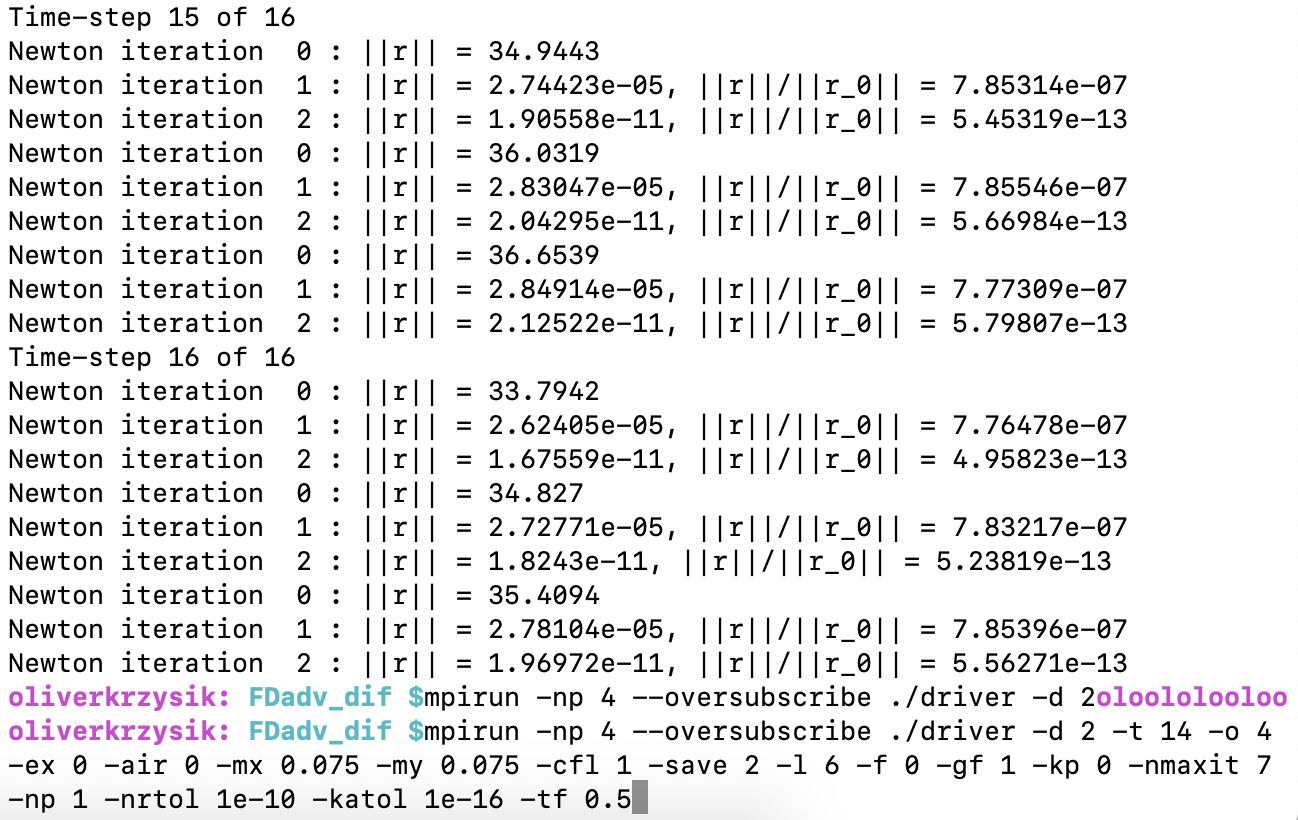
\includegraphics[width = 1\textwidth]{../figures/solves}
}
\caption{Newton convergence over last two time steps for the nonlinear problem in the bottom right panel of Figure \ref{fig:example}. Note the convergence on the 2nd iteration is quadratic.
\label{fig:solves}
}
\end{figure}

% ------------------------------------------------------------------------------- %
% \bibliographystyle{siamplain}
% \bibliography{refs.bib}


\end{document}

